%\documentclass{article}

%\usepackage{amsmath, amssymb, graphicx, multirow}

%\begin{document}

%\section{Introduction}

\section{Introduction and Motivation for RBF-FD}
\label{sec:rbf}

RBFs approximate a function $f(\mathbf{x}) \in \mathbb{R}^d$ sampled at $N$ distinct node locations by linearly combining translates of a single radially symmetric function, e.g. $\phi(r) = e^{-\varepsilon^2r^2}$, where $r=\|\mathbf{x}-\mathbf{x}_{i}\|$ denotes the Euclidean distance between where the function $f(\mathbf{x})$ is evaluated, $\mathbf{x}$, and where the RBF, $\phi$, is centered $\mathbf{x}_{i}$. The parameter $\varepsilon$ controls the shape of the RBF. Note that the argument of an RBF is simply a scalar distance $r$, independent of any coordinate system or dimension. As a result, nodes can be scattered as desired across complex physical domains with the implementation of the method being independent of dimensionality. Thus, no mesh generation is needed and algorithmic complexity does not increase with dimension.

To obtain a RBF derivative approximation at a node location that will result in a sparse differentiation matrix (DM), the RBF-FD method has been developed over the last decade \cite{TAI1,TAI2,SDY02,WrFo06}. RBF-FD is conceptually similar to standard finite differences (FD). However, the differentiation weights for approximating a derivative at a given node (forming one row of the RBF-FD derivative matrix) are derived from a function approxiation within the stencil formed by a linear combination of RBFs centered at the different points of the stencil. In general, $n<<N$. 
%that the linear combination of function values at the $n$ nearest node locations (a stencil) with $n \in N$ be exact for RBFs centered at each of the $n$ nodes rather than polynomials. 
The resulting derivative matrix (DM) is sparse matrix with $nN$ nonzero entries. As in FD methods, the order of the method increases with stencil size. An illustration of an RBF 32 node stencil on a sphere,  is given in Figure \ref{fig:stencil}.

\begin{figure}[t]
\centering
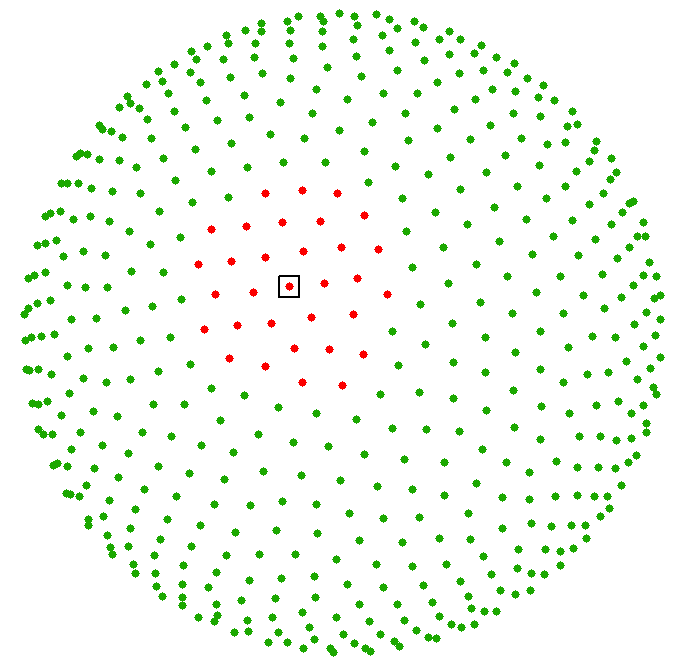
\includegraphics[width=0.8\linewidth]{figures/RBFStencil_n32_a}\label{fig:stencil}
\caption{An example of an RBF-FD stencil of size $n=32$ on a sphere of $N=1024$ nodes to approximate any derivative operator at the point in the square. In nonsparse format, the DM  is $1024\times1024$ with 21 nonzero entries per row.}
\end{figure}

Due to the above attributes and its simplicity of implementation, the RBF-FD is gaining popularity in modeling systems of PDEs in a variety of fields in fluid dynamics (e.g., geosciences, combustion, aerodynamics \cite{Bayona13,CDNT,FoL11,FLBWSC12,SPLM}). For example, the full shallow water equations in a 3D Cartesian coordinate system for a rotating fluid are as follows:
{
\small
\begin{eqnarray}
\dfrac{\partial u}{\partial t} &=& - \left( u\dfrac{\partial u}{\partial x} + v\dfrac{\partial u}{\partial y} + w\dfrac{\partial u}{\partial z} + f(yw - zv) + g\dfrac{\partial h}{\partial x} \right) 
\nonumber \\
\dfrac{\partial v}{\partial t} &=& - \left( u\dfrac{\partial v}{\partial x} + v\dfrac{\partial v}{\partial y} + w\dfrac{\partial v}{\partial z} + f(zu - xw) + g\dfrac{\partial h}{\partial x} \right)
\nonumber\\
\dfrac{\partial w}{\partial t} &=& - \left( u\dfrac{\partial w}{\partial x} + v\dfrac{\partial w}{\partial y} + w\dfrac{\partial w}{\partial z} + f(xv - yu) + g\dfrac{\partial h}{\partial x} \right)
\nonumber\\
\frac{\partial h}{\partial t}& =&-\left(\dfrac{\partial (uh)}{\partial x} + \dfrac{\partial (vh)}{\partial y} + h\dfrac{\partial (wh)}{\partial z}\right) , \label{height} \nonumber
\end{eqnarray}
} where $f$ is the Coriolis force, $\{u,v,w\}$ are the components of the velocity vector in the respective $\{x,y,z\}$ directions, and $h$ is the geopotential height (analogous to pressure). Thus, we have four variables $\{u,v,w,h\}$ and three DMs, $D_x, D_y, D_z$ representing $\dfrac{\partial}{\partial x}, \dfrac{\partial}{\partial y},\dfrac{\partial w}{\partial z}$, respectively. Moreover, in order to stably time step the equations with an explicit time-stepping scheme, most numerical methods (including RBF-FD) require a fourth operator, hyperviscosity, to be added to the each equation. Hyperviscosity takes the form of $\triangle^p$ ($\triangle$ denotes the Laplacian operator), where $p\geq3$, which is approximated by the matrix $D_{hyp}$. Therefore, in order to solve this system of PDEs, the application of 4 DM to 4 unknowns, i.e. 16 SpMV is required at every time step. Due to the fact that RBFs are independent of a coordinate system, taking into account only distances to nearest neighbors, the DMs have the following properties:
\begin{itemize}
\item For a given $n$, regardless of the operator approximated, e.g. $\dfrac{\partial}{\partial x}$ or the Laplacian, RBF-FD DMs will have the same number of nonzeros per row.
\item For a given $n$ and $N$, regardless of the operator approximated, the DMs will have the same sparsity pattern. Examples of an RBF-FD DM can be seen in Figures \ref{fig:spy_plots}d and e.
\end{itemize}

Multiple variables transform a SpMV into a SpMM (Sparse Matrix/dense Matrix multiplication), which improves register utilization and decreases cache
misses by vectorizing over the multiple source vectors. Furthermore, due to the properties just mentioned, multiple derivatives of a single function can be calculated rather than computing a single derivative of multiple functions. Using the PDE system above as an example, the block structure of the SpMM for computing all derivatives needed can be seen in Figure \ref{fig:struct_comp}, 
\begin{figure}[h]
  \centering
 {\small
  \[ \left( \begin{array}{cccc}
    \underline{u}_x     & \underline{v}_x     & \underline{w}_x     & \underline{h}_x \\
    \underline{u}_y     & \underline{v}_y     & \underline{w}_y     & \underline{h}_y \\
    \underline{u}_z     & \underline{v}_z     & \underline{w}_z     & \underline{h}_z \\
    \underline{u}_{hyp} & \underline{v}_{hyp} & \underline{w}_{hyp} & \underline{h}_{hyp}
  \end{array} \right)
  = \left(
  \begin{array}{c}
    D_{x}\\ D_{y}\\ D_{z}\\ D_{hyp}
  \end{array}\right)
  \times \left(\underline{u} \,\, \underline{v} \,\, \underline{w} \,\, \underline{h} \,\,\right) \]
 }
  \vspace{-1ex}
  \caption{Block structure of the computation.}
  \label{fig:struct_comp}
\end{figure}
where $\{\underline{u},\underline{v}, \underline{w}, \underline{h}\}$ are the functions values at all nodes of the corresponding variables with the left hand side being the resulting derivative approximations. The increased memory bandwidth due to an increase in the number of derivative matrices is offset by improved cache utilization, leading to an overall performance benefit. In practice however, the number of vectors whose derivatives are required is limited, capping the performance of the matrix/vector multiplication. Similarly, the number of different derivatives in a particular computation is finite. It is for this reason that we seek to combine the benefits of multiple vectors and multiple matrices simultaneously. We limit this initial study to four vectors and four matrices, which is a common number found in fluid dynamic calculations.

\ge{We also note that the DMs are time-independent. They are computed once and used repeatedly to update the solution 
in time. Thus, the cost to calculate the derivatives, although high, is amortized by the very long numerical simulations.}

%\end{document}
